%Beamer class
\documentclass{beamer}

\usepackage[czech]{babel}
\usepackage[cp1250]{inputenc}
\usepackage{fontenc}
\usepackage{tgheros}
\usepackage{array}
\usepackage{color}
\usepackage{hyperref}

\usetheme{Antibes}
\usecolortheme{crane}


\title[BE1M13VES]{BE1M13VES}
\subtitle[Manufacturing of Electrical Components] {Manufacturing of Electrical Components}
\author[Brejcha]{Michal Brejcha}
\institute[CTU]{CTU in Prague}
\date[Prague, 2017]{Prague, 2017}

\begin{document}
%------------------------------------------------------------------------------
%Uvodni slajd
%------------------------------------------------------------------------------
\frame{\titlepage}

\begin{frame}
\frametitle{Overview} 
\tableofcontents
\end{frame}

\AtBeginSection[]
{
  \begin{frame}
    \frametitle{TOPIC}
    \tableofcontents[currentsection]
  \end{frame}
}

%------------------------------------------------------------------------------
%Frquency dependency of resistors
%------------------------------------------------------------------------------
\section{\texorpdfstring{Semiconductor Components}{Semiconductor Components}}
%------------------------------------------------------------------------------
	\begin{frame}
    \frametitle{Semiconductor Components}
		\textbf{Basic properties}
		\begin{itemize}
		\item Nonlinear characteristics - used for rectifying, sensing, saturation etc.
		\item VA characteristics are quite dependent on ambient factors - temperature, light.
		\item Some components are able to amplify the input signal - transistors
		\end{itemize}
		
	\end{frame}
%------------------------------------------------------------------------------
	\begin{frame}
    \frametitle{Doping}
		\small
		\textbf{Intrinsic semiconductors (semiconductors without impurities):}
		
		\begin{itemize}
			\item The free charge is excited via temperature or light.
			\item Quite small conductivity dependent on ambient factors.
		\end{itemize}
		
		\textbf{Extrinsic semiconductors (semiconductors with doped material):}
		
		\begin{itemize}
			\item Most of the free charge is excited at room temperature from impurities.
			\item Similar behavior as metal conductors (rising resistance with temperature).
			\item Two types of doped materials (dopants): \textbf{\textcolor{brown}{donors \& acceptors}}
		\end{itemize}
		
	\end{frame}
%------------------------------------------------------------------------------
	\begin{frame}
    \frametitle{Doping}
		\small
		
		\textbf{Degenerate semiconductors}
		
		\begin{itemize}
			\item High level of dopant.
			\item Almost the same behaviour as metal conductors.
			\item Their are used to create contact layer between metal wire and semiconductor.
		\end{itemize}
		
		\textbf{Type of conduction}
		
		\begin{itemize}
			\item Adding donors (5 valence electrons) $\Rightarrow$ electrons conduction, type N (negative).
			\item Adding acceptors (3 valence electrons) $\Rightarrow$ holes conduction, type P (positive).
		\end{itemize}
	\end{frame}
%------------------------------------------------------------------------------
	\begin{frame}
    \frametitle{Temperature dependency}
		\begin{center}
			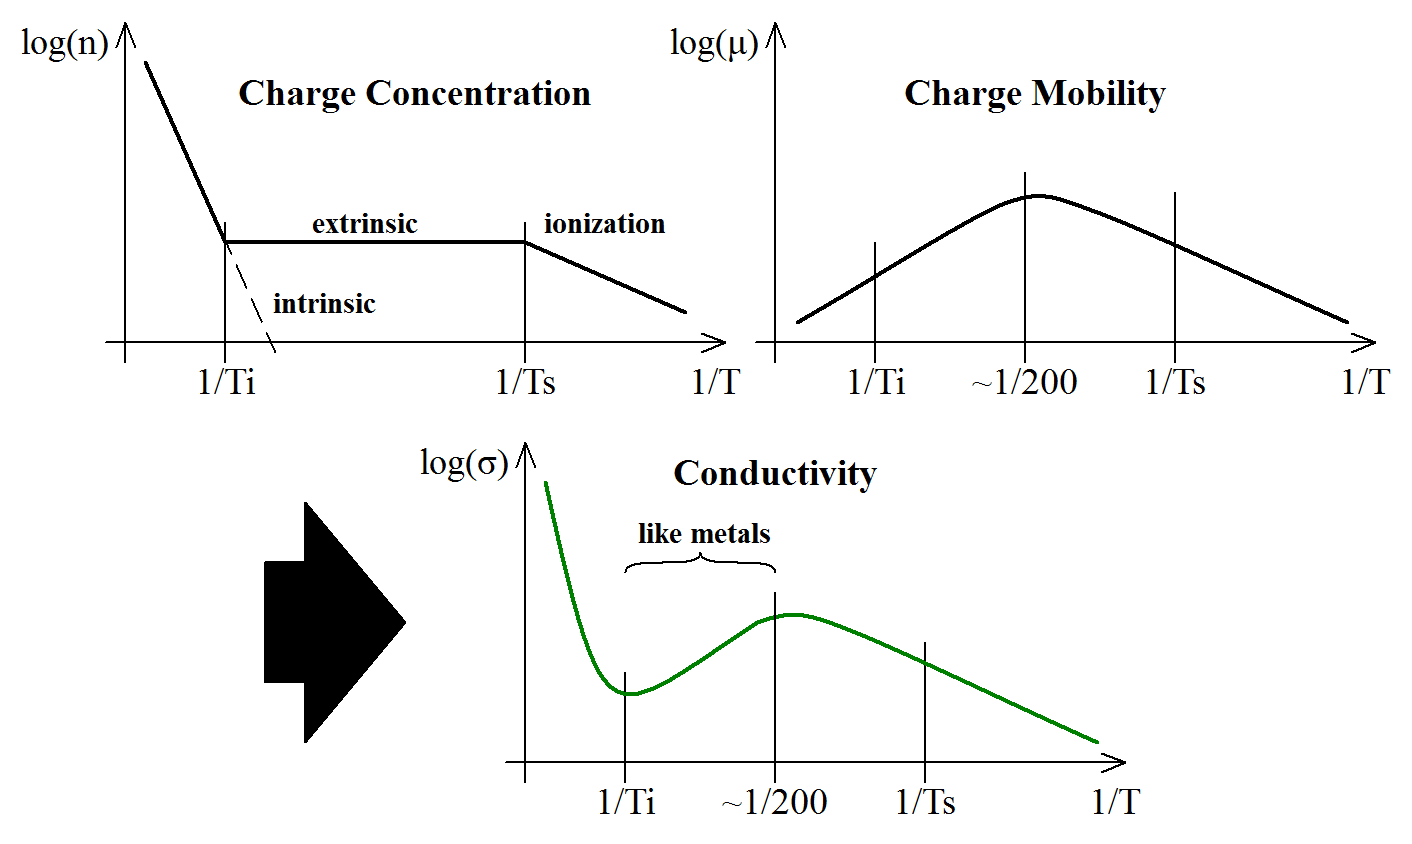
\includegraphics[scale=0.25]{obr02_tepZav.png}
		\end{center}
	\end{frame}
%------------------------------------------------------------------------------
	\begin{frame}
    \frametitle{Semiconductor Materials}
		\begin{center}
			\begin{tabular}{p{0.4\linewidth} p{0.5\linewidth}}
			\textbf{Element Materials:} & Si, Ge (old but still used in specific applications), ...(C, Sn $\Rightarrow$ IV. element group)\\
			\textbf{Compound materials:} & SiC (varistors and early LEDs), GaAs (LEDs), CdS (Photoresistors)\\
			\textbf{Donors:} & (V. element group) P, As\\
			\textbf{Acceptors:} & (III. element group) B, Al\\
			\end{tabular}
		\end{center}
	\end{frame}
%------------------------------------------------------------------------------
%Light Dependent Resistor
%------------------------------------------------------------------------------
\section{\texorpdfstring{Light Dependent Resistor}{Light Dependent Resistor}}
%------------------------------------------------------------------------------
	\begin{frame}
    \frametitle{LDR, Photoresistor - Basic properties}
		\small
		\begin{itemize}
		\item The resistance decreases with illumination.
		\item The spectral light sensitivity depends on semiconductor material.
		\end{itemize}
		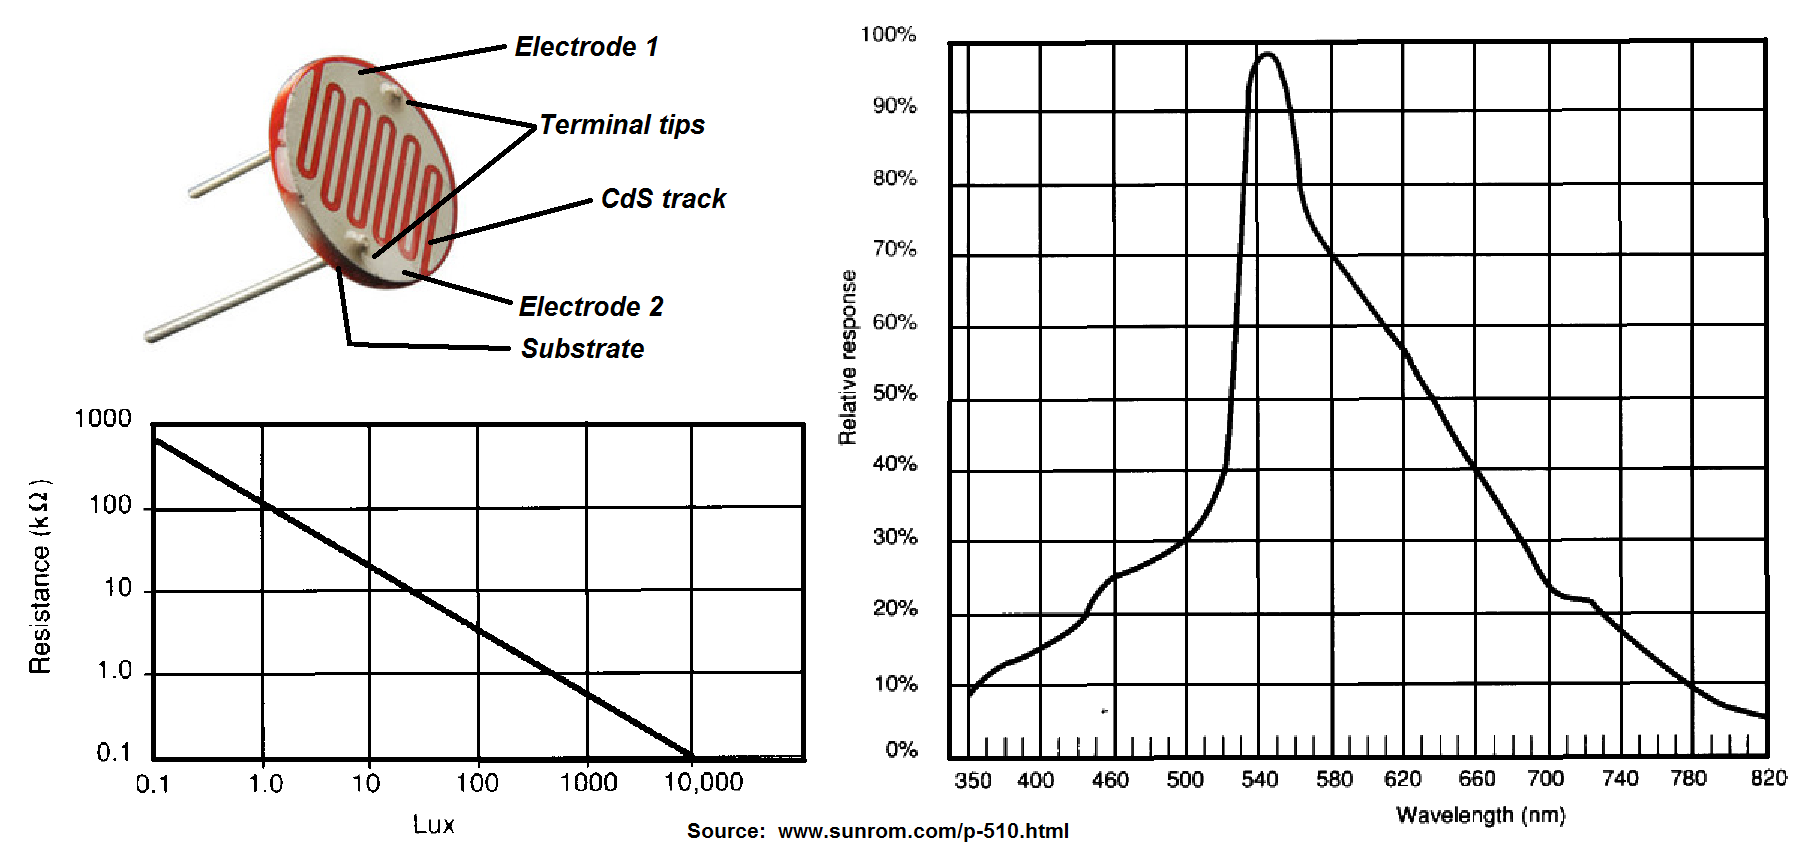
\includegraphics[scale=0.22]{obr01_fotoodpor.png}
	\end{frame}
%------------------------------------------------------------------------------
	\begin{frame}
    \frametitle{LDR Materials and dynamic features}
		\begin{center}
			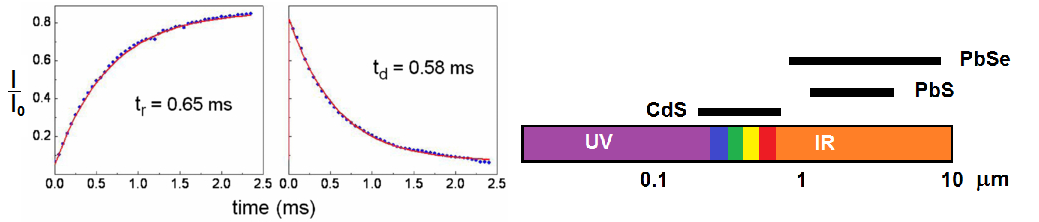
\includegraphics[scale=0.38]{obr03_materialyFO.png}
		\end{center}
		
		\begin{itemize}
		\item Materials: CdS, CdSe, PbS, PbSe, and others;
		\item \textbf{No PN junction} - one type of conductivity:
		\begin{itemize}
			\item intrinsic - high resistance, sensitive to short wavelengths of light
			\item extrinsic - smaller resistance, sensitive to longer wavelengths of light (IR)
		\end{itemize}
		\item Dynamic response is exponential: \textbf{miliseconds}
		\end{itemize}
	\end{frame}
%------------------------------------------------------------------------------
%Diodes
%------------------------------------------------------------------------------
\section{\texorpdfstring{Diodes}{Diodes}}
%------------------------------------------------------------------------------
	\begin{frame}
    \frametitle{Diode}
		The construction contain one junction between different types of semiconductor conductivity $\Rightarrow$ PN junction.
		\begin{center}
			\begin{tabular}{m{0.48\linewidth} m{0.42\linewidth}}
			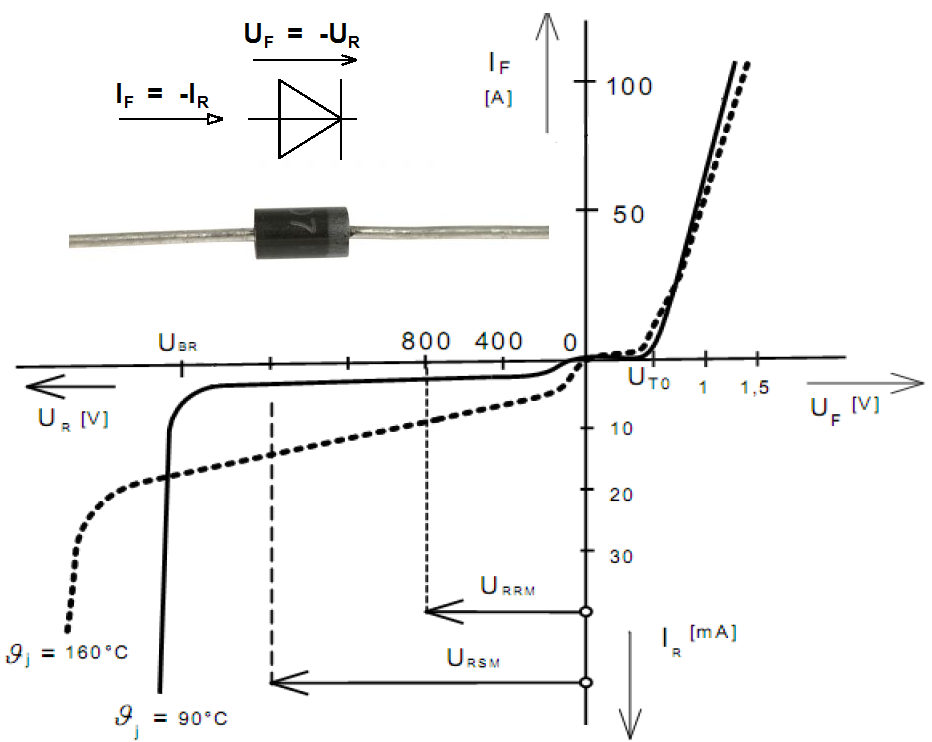
\includegraphics[scale=0.20]{obr04_dioda.png} &
			Shockley diode equation
			$$I = I_0\cdot\left(e^{\frac{U}{n\cdot U_T}}-1\right)$$
			\small
			\begin{itemize}
				\item[$I_0$] ... saturation current,
				\item[$U_T$] ...thermal voltage $=kT/e$,
				\item[$n$] ...emission coefficient $=\left\langle 1, 2\right\rangle$.
			\end{itemize}
			
			\end{tabular}
		\end{center}
	\end{frame}
%------------------------------------------------------------------------------
	\begin{frame}
    \frametitle{Diode - Forward Orientation}
		\begin{center}
			\begin{tabular}{m{0.60\linewidth} m{0.30\linewidth}}
			$$U_F\approx U_T + I\cdot r_T$$
			
			\begin{itemize}
				\item[$U_T$] threshold voltage, for Si diode $\approx 0.6$ V,
				\item[$r_T$] dynamic resistance.
			\end{itemize}
			$$r_T \approx \frac{\Delta U}{\Delta I} = \frac{3\cdot\Delta U}{2\cdot\Delta I_{FAV}}$$
			& 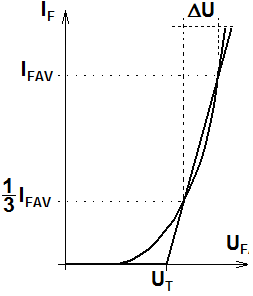
\includegraphics[scale=0.5]{obr10_propustnySmer} 
			\end{tabular}
		\end{center}
		Very small forward voltage and high reverse (breakdown) voltage are good properties for rectifying.
	\end{frame}
%------------------------------------------------------------------------------
	\begin{frame}
    \frametitle{Diode - Reverse Orientation}
		\begin{center}
			\begin{tabular}{m{0.55\linewidth} m{0.35\linewidth}}
			\small
			Breakdowns:
			
			\begin{enumerate}
				\item \textbf{electrical}... nondestructive, component handles the power loss (Zener diode and trisils).
				\item \textbf{thermal}... destructive, the power loss melts the semiconductor layer.
			\end{enumerate}
			Breakdown Mechanisms:
			
			\begin{enumerate}
				\item Avalanche - $U_{BR}$ icreases with temperature, in case $U_{BR} < 6$ V
				\item Quantum tunnelling - $U_{BR}$ decreases with temperature
			\end{enumerate}
			& 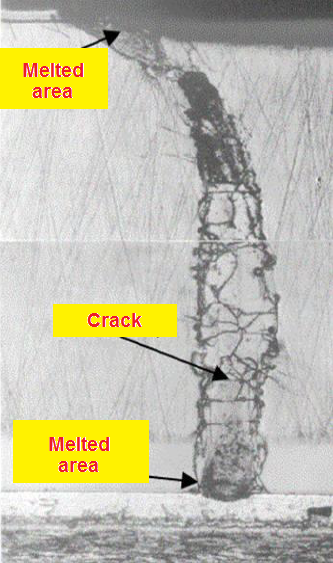
\includegraphics[scale=0.40]{obr05_tepPruraz.png} 
			\end{tabular}
		\end{center}
	\end{frame}
%------------------------------------------------------------------------------
	\begin{frame}
    \frametitle{Zener Diode and Trisil}
		\begin{center}
			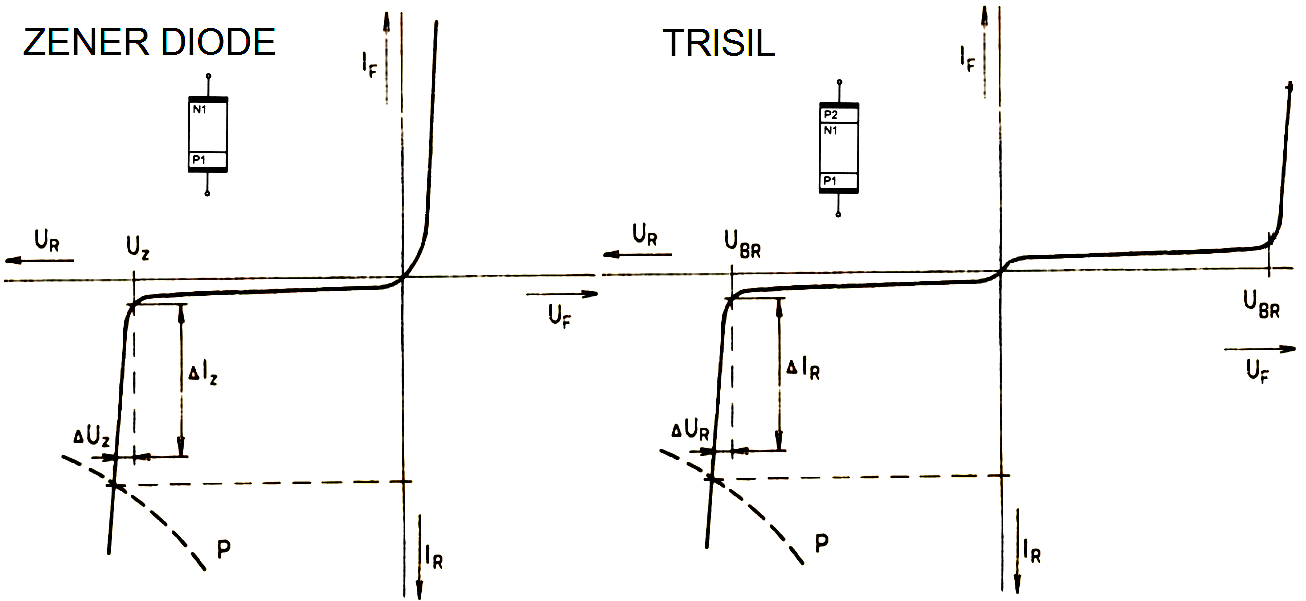
\includegraphics[scale=0.3]{obr06_zenerTrisil.png} 
		\end{center}
		\begin{tabular}{m{0.55\linewidth} m{0.35\linewidth}}
		\small
		They are used as voltage reference or protection (common voltages $\left\langle 2\:V, 200\:V\right\rangle$).
		 &
		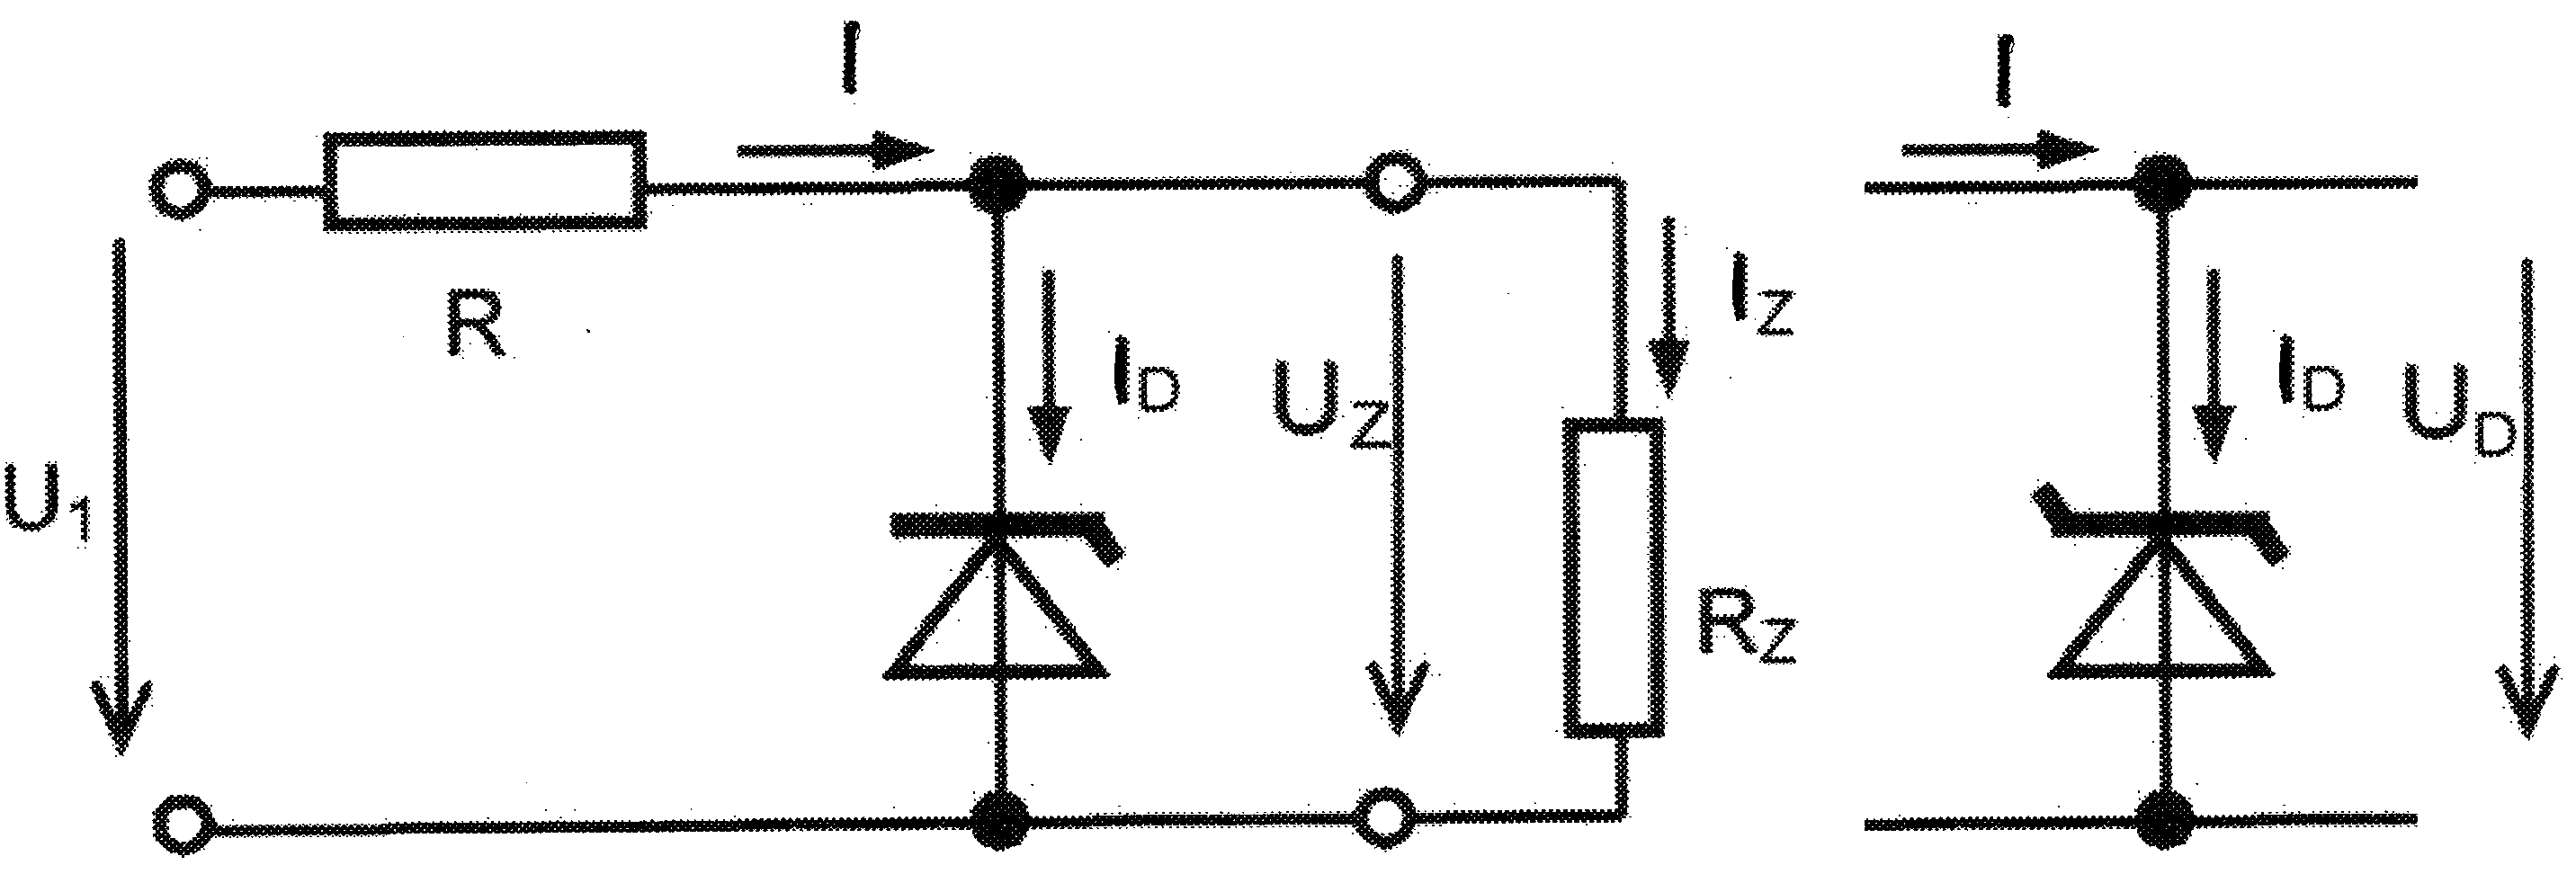
\includegraphics[scale=0.05]{obr09_zapojeniZener.png} 
		\end{tabular}
	\end{frame}
%------------------------------------------------------------------------------
	\begin{frame}
    \frametitle{Dynamic Behavior}
		\begin{tabular}{m{0.3\linewidth} m{0.6\linewidth}}
		Reverse Recovery:
		
		\begin{itemize}
			\item [$t_{rr}$] reverse recovery time
			\item [$t_{d}$] time of delay
			\item [$t_{f}$] time of fall
		\end{itemize}
		 &
		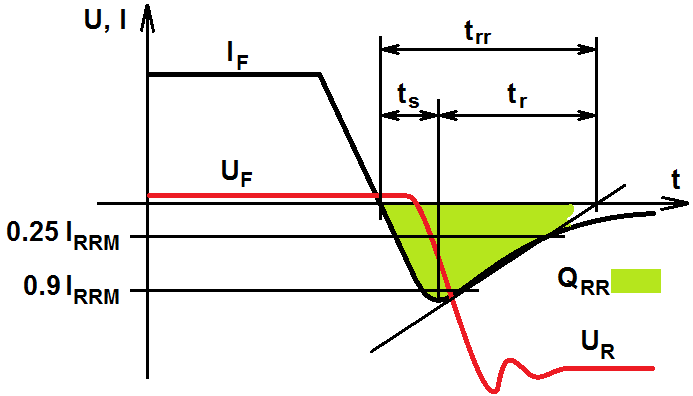
\includegraphics[scale=0.3]{obr07_zavZot.png} 
		\end{tabular}
		There is stored charge in the diode. The charge must be remove during the change of voltage polarity to recover reverse state of the diode.\\
		After approximation by a triangle: $$Q_{rr}=\frac{1}{2}\cdot I_{RRM}\cdot t_{rr}$$
	\end{frame}
%------------------------------------------------------------------------------
	\begin{frame}
    \frametitle{Schottky diode}
		\begin{tabular}{m{0.5\linewidth} m{0.4\linewidth}}
		\small
		\begin{itemize}
			\item Junction between semiconductor and metal.
			\item Smaller threshold voltage (0.3 V).
			\item Smaller recovery charge $Q_{rr}$ (fast).
			\item Smaller breakdown voltages (common max 50 V, rare up to 200 V)
		\end{itemize}
		 &
		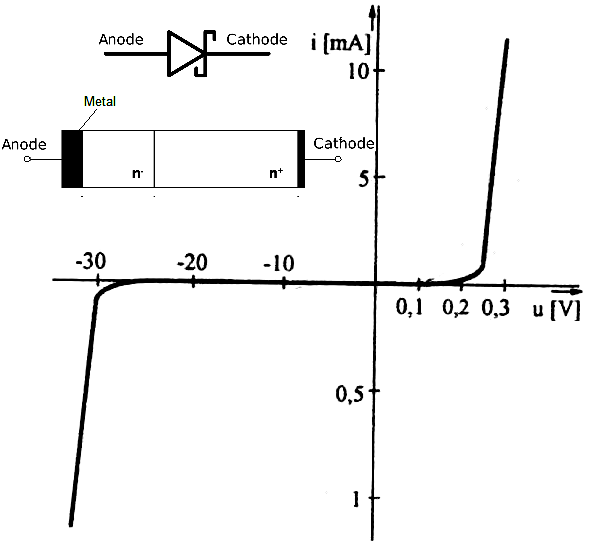
\includegraphics[scale=0.35]{obr12_schottkyDioda.png} 
		\end{tabular}
	\end{frame}
%------------------------------------------------------------------------------
	\begin{frame}
    \frametitle{Diodes - Technology}
		\begin{center}
			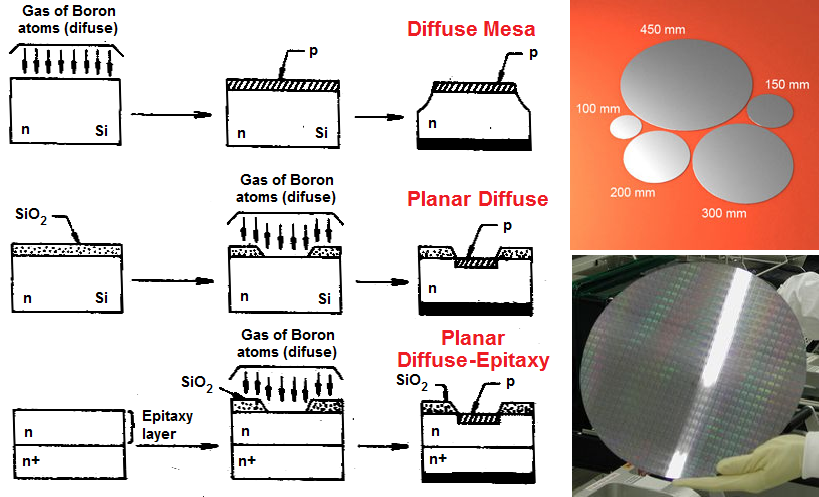
\includegraphics[scale=0.45]{obr11_vyrobaPN.png} 
		\end{center}
	\end{frame}
%------------------------------------------------------------------------------
%Transistors
%------------------------------------------------------------------------------
\section{\texorpdfstring{Transistors}{Transistors}}
%------------------------------------------------------------------------------
	\begin{frame}
    \frametitle{Bipolar Transistors - Basic Properties}
		\small
		Component with two PN junction and three electrodes:
		
		\begin{description}
			\item[BASE]... affect, control the current flow between COLLETOR and EMITTER
			\item[COLECTOR]... collects the electrons flowing through BASE.
			\item[EMITTER]... emits the electrons to the base.
		\end{description}
		\begin{tabular}{m{0.5\linewidth} m{0.4\linewidth}}
		\begin{flushleft}
			Arrangements: NPN, PNP
		\end{flushleft}
		\begin{flushleft}
			Applications: Amplifiers, switches
		\end{flushleft}
		 &
		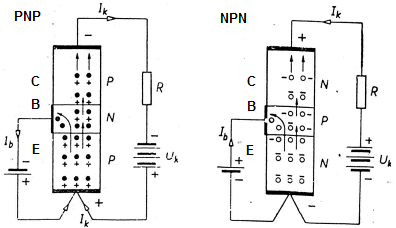
\includegraphics[scale=0.4]{obr13_pnpnpn.png} 
		\end{tabular}
	\end{frame}
%------------------------------------------------------------------------------
	\begin{frame}
    \frametitle{Transistors - Characteristics}
		\begin{center}
			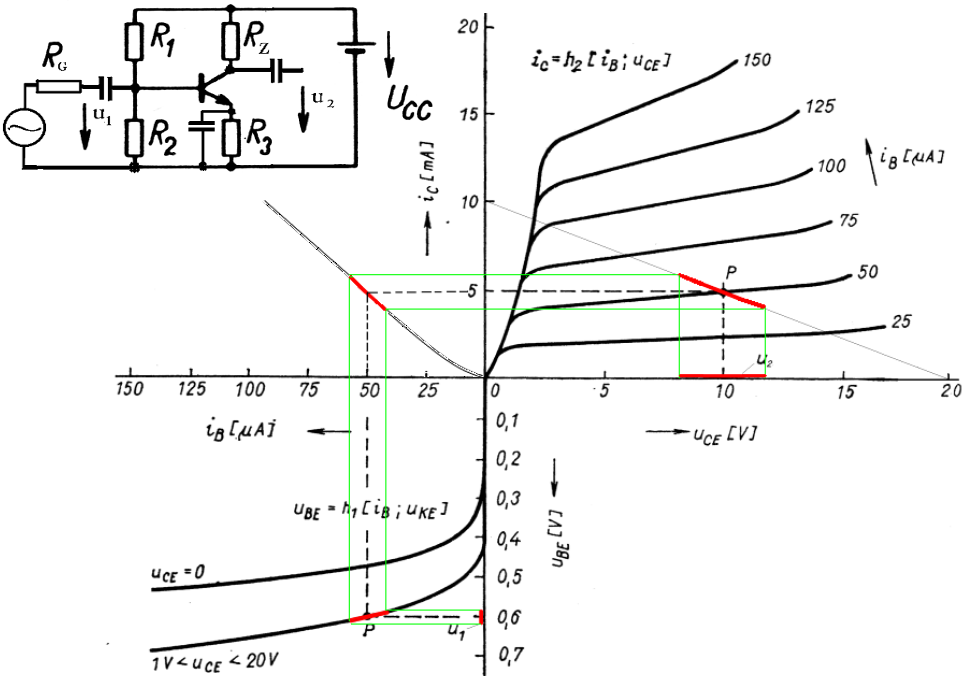
\includegraphics[scale=0.35]{obr08_charTranzistoru.png} 
		\end{center}
	\end{frame}
%------------------------------------------------------------------------------
	\begin{frame}
    \frametitle{Technology}
		Planar diffuse-epitaxy: epitaxy layer has thickness 10 $\mu$m and it is created on degenerated semiconductor (similar to diodes technology).
		\begin{tabular}{m{0.3\linewidth} m{0.6\linewidth}}
		\begin{center}
			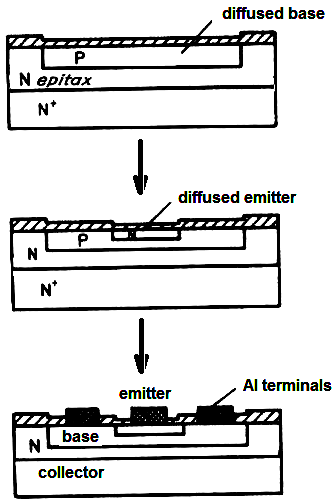
\includegraphics[scale=0.35]{obr14_npnTechnology.png} 
		\end{center} &
		
		\begin{enumerate}
			\item Creating the epitaxy N layer,
			\item diffuse of boron,
			\item creating of SiO$_2$ layer,
			\item mask etching,
			\item diffuse phosphor,
			\item another SiO$_2$ layer and etching,
			\item creating terminals.
		\end{enumerate}
		 
		\end{tabular}
	\end{frame}
%------------------------------------------------------------------------------
	\begin{frame}
    \frametitle{Structures}
		\small
		\begin{tabular}{m{0.5\linewidth} m{0.4\linewidth}}
		\begin{center}
			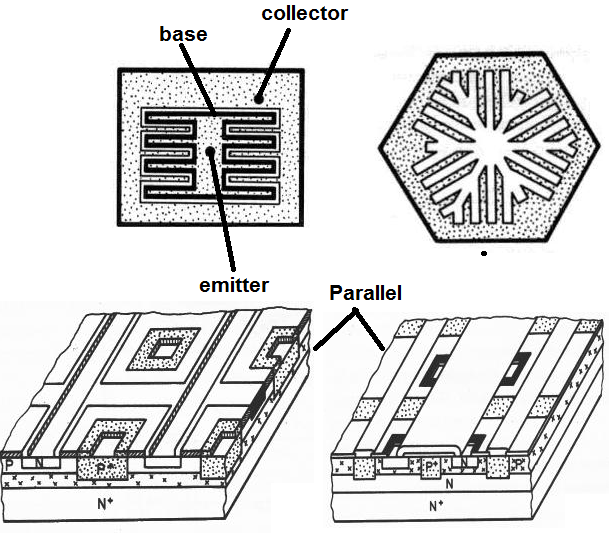
\includegraphics[scale=0.35]{obr15_npnStruktury.png} 
		\end{center} &
		
		The large emitter area is needed to get high current capability. The current density is the highest at the edge of emitter layer. Therefore the structures with long edge are preferred.
		 
		\end{tabular}
	\end{frame}
%------------------------------------------------------------------------------
	\begin{frame}
    \frametitle{Unipolar types}
		\begin{center}
			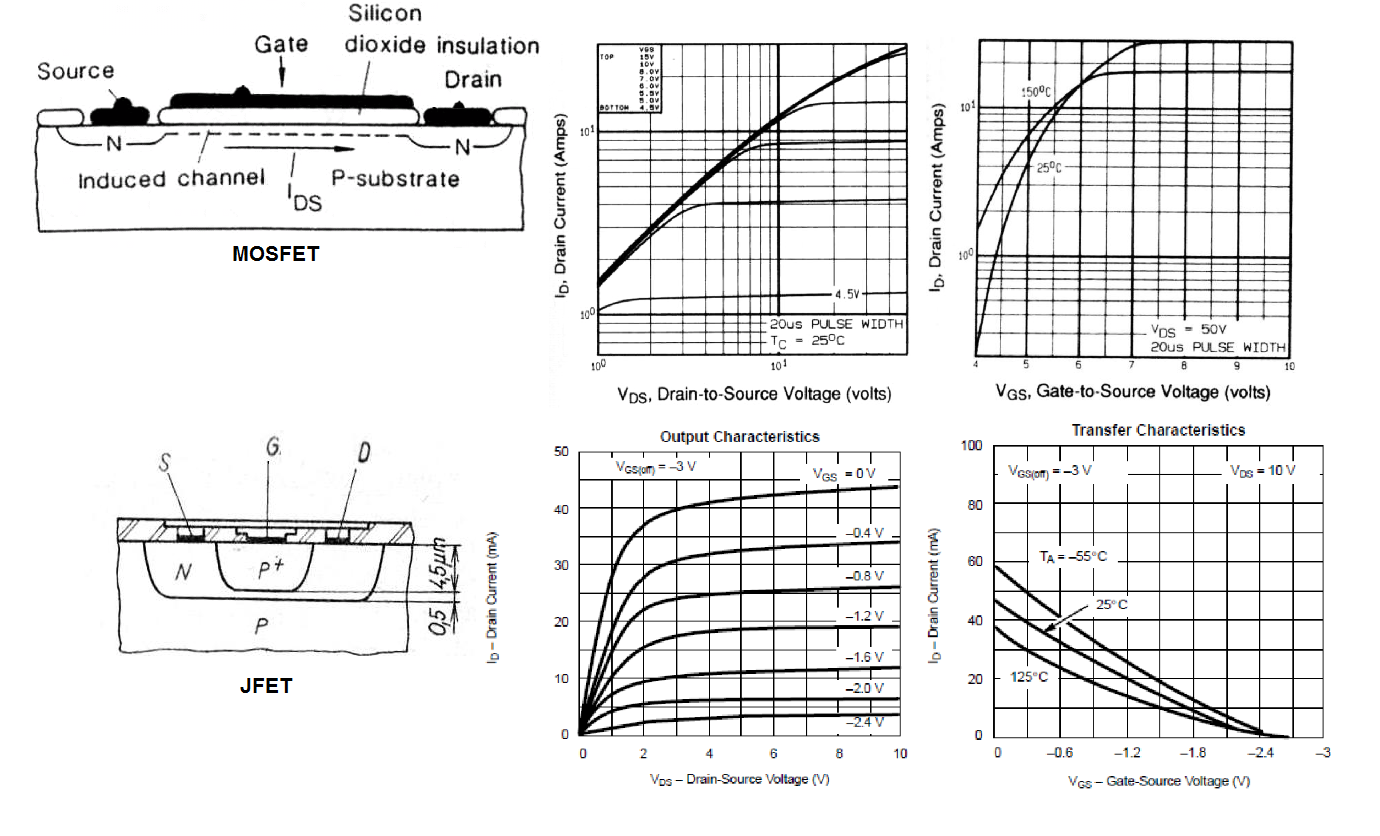
\includegraphics[scale=0.25]{obr16_mosTechnology.png} 
		\end{center}
		\small
		The flow of the current is controlled via electric field $\Rightarrow$ gate with low consumption.

	\end{frame}
%------------------------------------------------------------------------------
	\begin{frame}
    \frametitle{SIPMOS Technology}
		\begin{center}
			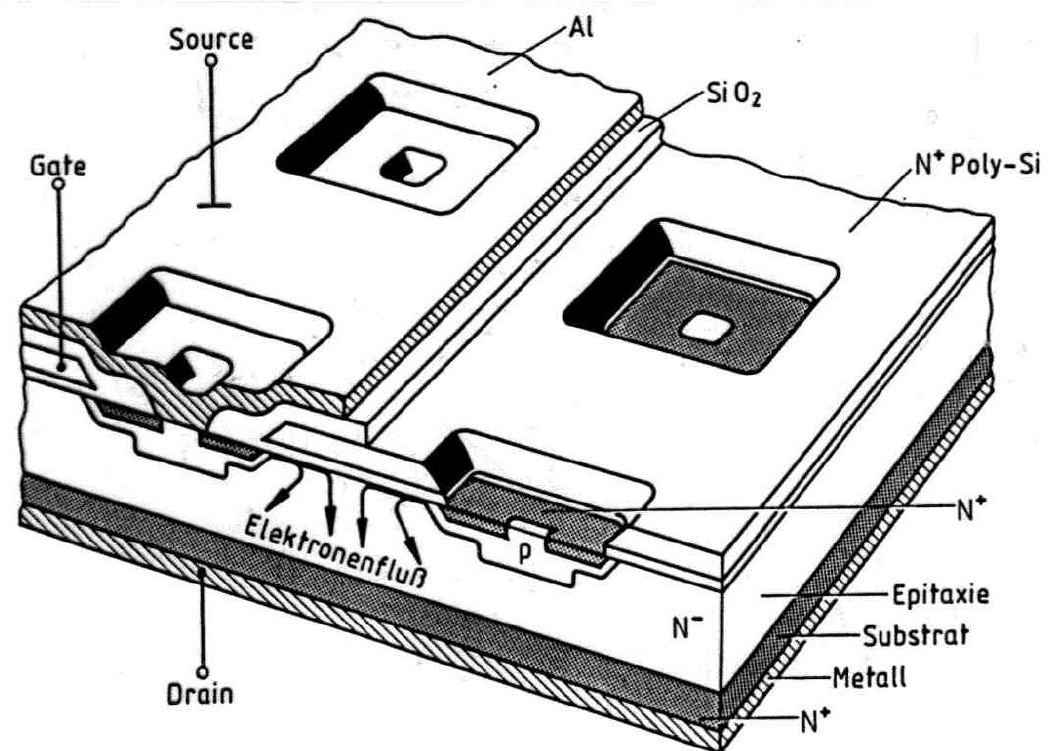
\includegraphics[scale=0.32]{obr17_sipmos.png} 
		\end{center}
	\end{frame}
%------------------------------------------------------------------------------
	\begin{frame}
    \frametitle{HEXFET Technology}
		\begin{center}
			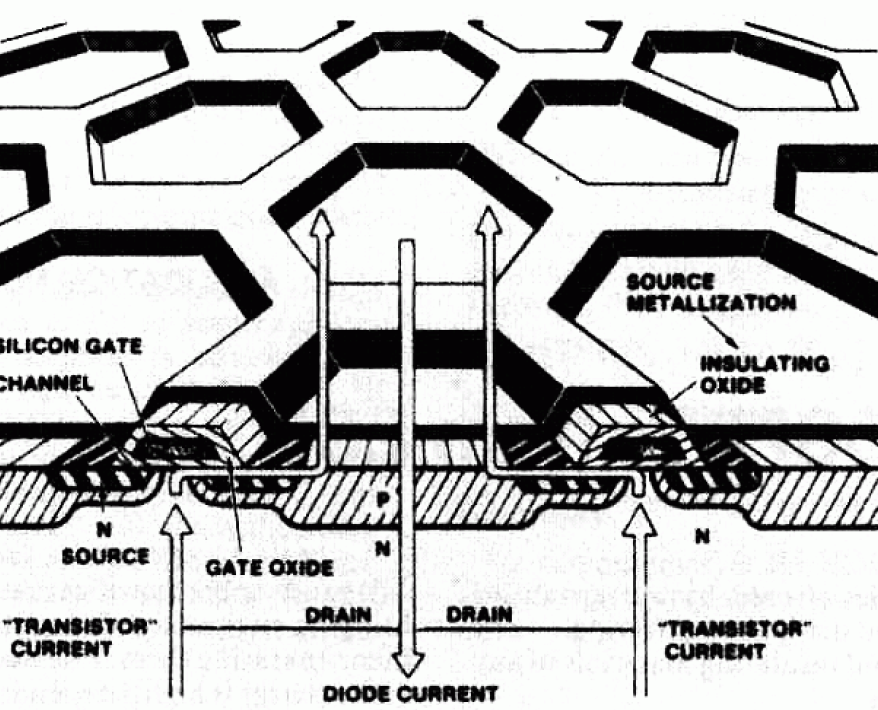
\includegraphics[scale=0.35]{obr18_hexfet.png} 
		\end{center}
	\end{frame}
%------------------------------------------------------------------------------
\end{document}